% !TEX program = xelatex

\documentclass[14pt,a4paper]{extreport}

\usepackage{fontspec}
\setmainfont{Times New Roman}[Ligatures=TeX]
\setsansfont{Arial}[Ligatures=TeX]
\setmonofont{Courier New}[Ligatures=TeX]

\usepackage{timcw}
\usepackage{array}
\usepackage{float}
\usepackage{xcolor}
\usepackage{listings}
\usepackage{caption}
\usepackage{tikz}
\usetikzlibrary{arrows.meta,positioning,shapes.geometric}
\geometry{left=25mm,right=15mm,top=20mm,bottom=20mm}
\renewcommand{\thechapter}{\arabic{chapter}}
\renewcommand{\thesection}{\thechapter.\arabic{section}}
\renewcommand{\thesubsection}{\thesection.\arabic{subsection}}
\renewcommand{\thefigure}{\thechapter.\arabic{figure}}
\captionsetup[figure]{name={Рис.},labelsep=space}
\emergencystretch=3em
\sloppy
\titleformat{\chapter}
  {\fontsize{16pt}{16pt}\bfseries\centering}
  {\chaptername\ \thechapter}
  {1em}
  {}
\titlespacing*{\chapter}{0pt}{0pt}{18pt}
\makeatletter
\renewcommand{\@seccntformat}[1]{\csname the#1\endcsname\quad}
\makeatother
\renewcommand{\cftchapaftersnum}{\ }

\lstdefinestyle{pythoncode}{
  language=Python,
  basicstyle=\small\ttfamily,
  keywordstyle=\bfseries,
  commentstyle=\itshape\color{gray},
  stringstyle=\color{black},
  breaklines=true,
  columns=fullflexible,
  frame=single,
  showstringspaces=false,
  tabsize=4
}

\newcommand{\projecttitle}{Разработка информационной системы учета продуктов питания с анализом чеков и контролем сроков годности}

\newcommand{\maketitlepage}{%
\begin{titlepage}
\thispagestyle{empty}
\noindent
\begin{minipage}[c]{0.12\textwidth}
  
\includegraphics[width=0.82\linewidth]{tim-logo.png}
\end{minipage}%
\hfill
\begin{minipage}[c]{0.84\textwidth}
  \begin{center}
  \scriptsize
  \textbf{МИНИСТЕРСТВО СЕЛЬСКОГО ХОЗЯЙСТВА РОССИЙСКОЙ ФЕДЕРАЦИИ}\\[0.08cm]
  ФЕДЕРАЛЬНОЕ ГОСУДАРСТВЕННОЕ БЮДЖЕТНОЕ ОБРАЗОВАТЕЛЬНОЕ УЧРЕЖДЕНИЕ ВЫСШЕГО ОБРАЗОВАНИЯ\\[0.08cm]
  \textbf{«РОССИЙСКИЙ ГОСУДАРСТВЕННЫЙ АГРАРНЫЙ УНИВЕРСИТЕТ -- МСХА имени К.\,А.~ТИМИРЯЗЕВА»}\\[0.08cm]
  \textbf{(ФГБОУ ВО РГАУ -- МСХА имени К.\,А.~Тимирязева)}
  \end{center}
\end{minipage}

\vspace{0.08cm}
\noindent\rule{\textwidth}{0.4pt}\\[-2.1ex]
\rule{\textwidth}{0.4pt}

\begin{center}
\small
Институт экономики и управления\\
Кафедра статистики и кибернетики\\[0.1cm]
Направление: 09.03.02 «Информационные системы и технологии»\\
Направленность: «Компьютерные науки и информационный анализ данных»\\[0.1cm]
Методы и средства проектирования информационных систем и технологий\\[0.25cm]
{\normalsize\textbf{КУРСОВОЙ ПРОЕКТ}}
\end{center}

\vspace{0.05cm}
\noindent на тему: «\projecttitle».\\[0.12cm]

\hfill
\begin{minipage}[t]{0.56\textwidth}
Выполнила:\\
Студент 3 курса группы Д-Э 341\\
Нгуен Фыонг Ань\\[0.14cm]

Дата регистрации КП\\
на кафедре: \rule{4.5cm}{0.4pt}\\[0.08cm]

Допущен к защите\\[0.06cm]
Руководитель:\\
Доцент, Калитвин Владимир Анатольевич\\
\rule{6.5cm}{0.4pt}\\
{\small подпись}\\[0.08cm]

Члены комиссии:\\[0.05cm]
\rule{4.8cm}{0.4pt}\hfill\rule{1.6cm}{0.4pt}\\[-2pt]
{\footnotesize учёная степень, учёное звание, ФИО}\hfill{\footnotesize подпись}\\[0.04cm]
\rule{4.8cm}{0.4pt}\hfill\rule{1.6cm}{0.4pt}\\[-2pt]
{\footnotesize учёная степень, учёное звание, ФИО}\hfill{\footnotesize подпись}\\[0.04cm]
\rule{4.8cm}{0.4pt}\hfill\rule{1.6cm}{0.4pt}\\[-2pt]
{\footnotesize учёная степень, учёное звание, ФИО}\hfill{\footnotesize подпись}\\[0.06cm]

Оценка \rule{4.8cm}{0.4pt}\\[0.08cm]
Дата защиты \rule{4.4cm}{0.4pt}
\end{minipage}

\vfill
\begin{center}
Москва, 2026
\end{center}
\end{titlepage}
}

\newcommand{\makeassignmentpage}{%
\begin{titlepage}
\thispagestyle{empty}
\begin{center}
МИНИСТЕРСТВО СЕЛЬСКОГО ХОЗЯЙСТВА\\
РОССИЙСКОЙ ФЕДЕРАЦИИ\\[0.1cm]
Российский государственный аграрный университет -- МСХА\\
имени К.\,А.~Тимирязева\\[0.3cm]
Институт экономики и управления\\
Кафедра статистики и кибернетики\\[0.45cm]
{\fontsize{12pt}{14pt}\selectfont\textbf{ЗАДАНИЕ}}\\
{\fontsize{12pt}{14pt}\selectfont\textbf{НА КУРСОВОЙ ПРОЕКТ (КП)}}
\end{center}

\vspace{0.1cm}
\noindent \textbf{Обучающийся}\hrulefill\\[0.08cm]
\noindent \textbf{Тема КП} \hrulefill\\[0.08cm]
\noindent\rule{\textwidth}{0.4pt}\\[0.18cm]

\noindent Исходные данные к работе\hrulefill\\[0.08cm]
\noindent\rule{\textwidth}{0.4pt}\\[0.08cm]
\noindent\rule{\textwidth}{0.4pt}\\[0.08cm]
\noindent\rule{0.88\textwidth}{0.4pt}\\[0.18cm]

\noindent Перечень подлежащих разработке в работе вопросов:\\[0.06cm]
\noindent\rule{\textwidth}{0.4pt}\\[0.08cm]
\noindent\rule{\textwidth}{0.4pt}\\[0.08cm]
\noindent\rule{\textwidth}{0.4pt}\\[0.08cm]
\noindent\rule{\textwidth}{0.4pt}\\[0.08cm]
\noindent\rule{\textwidth}{0.4pt}\\[0.08cm]
\noindent\rule{\textwidth}{0.4pt}\\[0.08cm]
\noindent\rule{\textwidth}{0.4pt}\\[0.08cm]
\noindent\rule{0.78\textwidth}{0.4pt}\\[0.18cm]

\noindent Перечень дополнительного материала\hrulefill\\[0.08cm]
\noindent\rule{\textwidth}{0.4pt}\\[0.08cm]
\noindent\rule{\textwidth}{0.4pt}\\[0.08cm]
\noindent\rule{0.88\textwidth}{0.4pt}\\[0.24cm]

\noindent Дата выдачи задания \hfill «\rule{0.7cm}{0.4pt}»\rule{3.2cm}{0.4pt}202\_\_г.\\[0.18cm]
\noindent Руководитель (подпись, ФИО) \hfill \rule{5.0cm}{0.4pt}\\[0.18cm]
\noindent Задание принял к исполнению (подпись обучающегося) \hfill \rule{5.0cm}{0.4pt}\\[0.1cm]
\noindent\hfill «\rule{0.7cm}{0.4pt}»\rule{3.2cm}{0.4pt}202\_\_г.
\end{titlepage}
}

\begin{document}
\renewcommand{\thechapter}{\arabic{chapter}}
\renewcommand{\thesection}{\thechapter.\arabic{section}}
\renewcommand{\thesubsection}{\thesection.\arabic{subsection}}
\makeatletter
\def\postchapter{}
\def\postsection{}
\def\@seccntformat#1{\csname the#1\endcsname\quad}
\def\@tocseccntformat#1{\csname the#1\endcsname}
\makeatother
\begin{singlespacing}
\maketitlepage
\makeassignmentpage

\setcounter{page}{3}
\renewcommand{\contentsname}{\hfill Содержание\hfill}
\tableofcontents
\end{singlespacing}
\newpage

\intro

Современные домашние хозяйства и малые организации сталкиваются с задачей регулярного контроля запасов продуктов питания. При отсутствии систематизированного учета пользователь часто не имеет полной информации о составе запасов, сроках годности и необходимости своевременного использования продуктов. Это приводит к финансовым потерям, росту пищевых отходов и снижению качества планирования покупок. Дополнительную сложность создает то, что сведения о покупке обычно содержатся в кассовых чеках, электронных письмах и сообщениях от магазинов, то есть в слабоструктурированных источниках.

Актуальность темы обусловлена необходимостью разработки прикладной информационной системы, которая объединяет учет продуктов, импорт данных из чеков, определение сроков хранения и уведомление пользователя о приближении даты истечения срока годности. В рамках данной работы рассматривается программный проект Smart Fridge, реализованный на языке Python с использованием фреймворка Django и базы данных PostgreSQL.

Цель курсового проекта -- разработать и описать информационную систему учета продуктов питания с анализом чеков и контролем сроков годности.

Для достижения поставленной цели необходимо решить следующие задачи:
\begin{itemize}
  \item проанализировать предметную область учета продуктов питания и контроля сроков годности;
  \item определить функциональные и нефункциональные требования к информационной системе;
  \item описать архитектуру Django-приложения Smart Fridge и структуру его модулей;
  \item рассмотреть алгоритмы парсинга чеков, классификации продуктовых позиций, подбора срока хранения и формирования уведомлений;
  \item описать результаты тестирования ключевых сценариев работы системы.
\end{itemize}

Объектом исследования является процесс учета продуктов питания и контроля сроков годности. Предметом исследования являются методы проектирования и программной реализации веб-ориентированной информационной системы для автоматизации указанного процесса.

Практическая значимость работы состоит в том, что разработанное приложение может использоваться как прототип персональной системы управления продуктовым запасом, а также как учебный пример построения монолитного веб-приложения на Django с обработкой данных из внешних источников.

\newpage
\chapter[Глава \thechapter Теоретическая часть]{Теоретическая часть}

\section{Информационные системы учета продуктов питания}

Информационная система учета продуктов питания представляет собой совокупность программных средств, данных и процедур, обеспечивающих регистрацию продуктовых запасов, хранение сведений о количестве, категориях, датах покупки и сроках годности. В отличие от простого списка покупок такая система должна поддерживать жизненный цикл продукта: появление в запасах, уточнение параметров хранения, контроль состояния и удаление после использования.

В предметной области домашнего учета продуктов можно выделить следующие сущности: пользователь, продукт, категория, источник поступления данных, правило срока хранения и уведомление. Пользователь создает или импортирует записи о продуктах. Категория позволяет группировать товары по смысловым признакам, например молочные продукты, хлеб, крупы или напитки. Источник данных показывает, каким способом продукт был добавлен: вручную, из текстового чека, из файла или из письма. Правило срока хранения задает ожидаемую длительность безопасного хранения продукта. Уведомление информирует пользователя о необходимости обратить внимание на продукт.

Для таких систем важны не только операции CRUD, но и качество входных данных. Реальные чеки и письма часто содержат служебные строки, HTML-разметку, сведения о кассе, оплате, рекламе и доставке. Поэтому информационная система должна отделять продуктовые позиции от шумовых данных, нормализовать единицы измерения и предотвращать повторный импорт уже обработанных источников.

\section{Анализ чеков и извлечение товарных позиций}

Кассовый чек является полуструктурированным документом. Он содержит строки товаров, количество, цену, налоговые реквизиты, итоговые суммы и служебную информацию. При обработке бумажных чеков часто используется OCR -- оптическое распознавание символов. В результате OCR изображение преобразуется в текст, однако полученный текст может содержать ошибки распознавания, лишние переносы строк и неточные пробелы \cite{ocrbook}.

В электронных чеках и письмах часть проблем OCR отсутствует, но возникает другая задача: извлечение текста из HTML-писем, фильтрация служебной разметки, определение релевантных писем и защита от повторной обработки. Поэтому в учебной реализации целесообразно использовать комбинированный подход: ручная вставка текста, загрузка файла с последующей возможностью ручной корректировки, а также IMAP-импорт писем.

Для выделения товарных позиций применяются регулярные выражения, словари признаков и простые правила классификации. Регулярное выражение позволяет найти строки вида ``название -- количество -- единица измерения -- цена''. Словарь продуктовых слов помогает отличать пищевые товары от непищевых, например исключать пакеты, салфетки, бытовую химию или косметику.

\section{Контроль сроков годности}

Срок годности продукта определяется совокупностью факторов: типом продукта, условиями хранения, датой покупки и индивидуальными свойствами товара. В информационной системе срок хранения может задаваться пользователем вручную либо подбираться автоматически на основе базы знаний. База знаний представляет собой набор правил, где каждому названию или категории продукта соответствует количество дней хранения и условия хранения.

Автоматический подбор срока хранения может выполняться по точному совпадению названия или по оценке похожести. Если точного совпадения нет, система сравнивает название продукта с описаниями и тегами правил. Такая процедура не гарантирует абсолютной точности, поэтому продукты с неопределенным сроком должны получать статус, требующий подтверждения пользователем.

Контроль срока годности реализуется через вычисление даты окончания хранения:
\[
  D_{exp} = D_{purchase} + L,
\]
где \(D_{exp}\) -- дата истечения срока годности, \(D_{purchase}\) -- дата покупки, \(L\) -- срок хранения в днях. На основе этой даты система определяет состояние продукта: свежий, скоро истекает, просрочен или требует подтверждения.

\begin{figure}[H]
\centering
\begin{tikzpicture}[
  node distance=1.7cm,
  stage/.style={rectangle, rounded corners, draw, align=center, minimum width=3.0cm, minimum height=0.9cm},
  arrow/.style={-{Stealth[length=3mm]}, thick}
]
\node[stage] (add) {Добавление\\продукта};
\node[stage, right=of add] (shelf) {Определение\\срока хранения};
\node[stage, right=of shelf] (status) {Расчет\\статуса};
\node[stage, below=of status] (notify) {Формирование\\уведомления};
\node[stage, left=of notify] (use) {Использование\\или удаление};
\draw[arrow] (add) -- (shelf);
\draw[arrow] (shelf) -- (status);
\draw[arrow] (status) -- (notify);
\draw[arrow] (notify) -- (use);
\draw[arrow] (use) -- (add);
\end{tikzpicture}
\caption{Жизненный цикл записи о продукте в системе}
\end{figure}

\newpage
\chapter[Глава \thechapter Аналитическая часть]{Аналитическая часть}

\section{Постановка задачи}

Разрабатываемая система предназначена для автоматизации учета продуктов питания. Пользователь должен иметь возможность регистрироваться, добавлять продукты вручную, импортировать продукты из текста чека или письма, просматривать текущие запасы и получать уведомления о приближении срока годности.

Основная проблема предметной области состоит в том, что данные о покупке продуктов поступают из неоднородных источников. Пользователь может иметь бумажный чек, электронный чек, письмо от магазина или собственный текстовый список. При этом система должна работать без обязательного подключения внешних коммерческих API, чтобы оставаться доступной и воспроизводимой в учебной среде.

\section{Функциональные требования}

Функциональные требования к системе представлены ниже.
\begin{enumerate}
  \item[F1.] Пользователь должен иметь возможность зарегистрироваться, войти в систему и редактировать профиль.
  \item[F2.] Пользователь должен иметь возможность добавлять, редактировать и удалять продукты питания.
  \item[F3.] Система должна поддерживать импорт продуктов из текстового представления чека.
  \item[F4.] Система должна поддерживать загрузку файла чека и ручное уточнение распознанного текста.
  \item[F5.] Система должна поддерживать настройку IMAP-источника электронной почты и импорт писем с чеками.
  \item[F6.] Система должна выделять из текста только пищевые товары и игнорировать очевидные непищевые позиции.
  \item[F7.] Система должна подбирать срок хранения продукта на основе базы знаний.
  \item[F8.] Система должна формировать уведомления за 3 дня, за 1 день и после истечения срока годности.
  \item[F9.] Пользователь должен иметь возможность управлять пользовательскими правилами сроков хранения.
\end{enumerate}

\section{Нефункциональные требования}

К нефункциональным требованиям относятся:
\begin{itemize}
  \item безопасность пользовательских страниц за счет обязательной аутентификации;
  \item защита HTML-форм от CSRF-атак стандартными средствами Django;
  \item хранение секретных параметров подключения во внешнем файле окружения;
  \item устойчивость импорта к ошибкам OCR, отсутствию внешних API и недоступности почтового сервера;
  \item возможность запуска в локальной среде без Celery, Redis и дополнительных фоновых сервисов;
  \item совместимость с PostgreSQL как основной реляционной СУБД.
\end{itemize}

\section{Выбор архитектурного подхода}

Для реализации выбран монолитный подход на Django. Такой подход соответствует масштабу учебного проекта: все основные функции находятся в одном приложении, но разделены по Django-приложениям. Монолит упрощает развертывание, миграции базы данных, тестирование и навигацию по коду. При этом логическое разделение на модули сохраняет возможность последующего расширения.

Основные приложения проекта:
\begin{itemize}
  \item \texttt{accounts} -- регистрация, профиль пользователя и настройки уведомлений;
  \item \texttt{pantry} -- учет продуктов и категорий;
  \item \texttt{receipts} -- обработка чеков, файлов и почтового импорта;
  \item \texttt{knowledge} -- база знаний сроков хранения;
  \item \texttt{notifications} -- создание и отображение уведомлений.
\end{itemize}

\begin{figure}[H]
\centering
\begin{tikzpicture}[
  node distance=1.3cm and 1.7cm,
  comp/.style={rectangle, draw, rounded corners, align=center, minimum width=3.2cm, minimum height=0.9cm},
  store/.style={cylinder, draw, shape border rotate=90, aspect=0.25, align=center, minimum width=2.2cm, minimum height=1.1cm},
  arrow/.style={-{Stealth[length=3mm]}, thick}
]
\node[comp] (browser) {Браузер\\пользователя};
\node[comp, right=of browser] (views) {Django Views\\и Forms};
\node[comp, right=of views] (services) {Сервисный\\слой};
\node[store, below=of services] (db) {PostgreSQL};
\node[comp, above=of services] (imap) {IMAP-сервер\\почты};
\node[comp, below=of views] (templates) {Django\\Templates};
\draw[arrow] (browser) -- (views);
\draw[arrow] (views) -- (services);
\draw[arrow] (views) -- (templates);
\draw[arrow] (templates) -- (browser);
\draw[arrow] (services) -- (db);
\draw[arrow] (services) -- (imap);
\draw[arrow] (imap) -- (services);
\end{tikzpicture}
\caption{Компонентная архитектура приложения Smart Fridge}
\end{figure}

\section{Модель данных}

В базе данных используются связанные сущности. Центральной сущностью является \texttt{Product}, содержащая название продукта, количество, единицу измерения, категорию, дату покупки, срок хранения, дату истечения и статус. Сущность \texttt{Receipt} хранит исходный текст чека или письма, а \texttt{ReceiptItem} фиксирует распознанные позиции. Модель \texttt{EmailImportSource} задает параметры подключения к IMAP-серверу, а \texttt{ProcessingLog} предотвращает повторный импорт одного и того же письма.

База знаний представлена моделью \texttt{ShelfLifeRule}. Правила могут быть общими или принадлежать конкретному пользователю. Уведомления представлены моделью \texttt{Notification}; для предотвращения дублей используется уникальность пары ``продукт -- тип уведомления''.

\newpage
\chapter[Глава \thechapter Практическая часть]{Практическая часть}

\section{Общая характеристика программной реализации}

Проект Smart Fridge реализован на Python 3.11+ с использованием Django 5.x. В качестве СУБД используется PostgreSQL. Пользовательский интерфейс построен на Django Templates, HTML-формах и базовых CSS-стилях. Для работы с электронной почтой используется стандартная библиотека Python \texttt{imaplib}; для HTTP-интеграций OCR и LLM предусмотрен модуль \texttt{urllib.request}. В проекте сознательно не используются Flask, FastAPI, Django REST Framework, Node.js, React, Vue, Celery, Redis и RabbitMQ.

Структура проекта соответствует типовой организации Django-монолита:
\begin{itemize}
  \item каталог \texttt{smart\_fridge} содержит настройки и корневые маршруты;
  \item каталог \texttt{templates} содержит HTML-шаблоны страниц;
  \item каталог \texttt{static/css} содержит базовые стили интерфейса;
  \item каталог \texttt{tests} содержит тесты ключевых пользовательских сценариев.
\end{itemize}

Практическая проверка выполнялась на запущенном локальном экземпляре приложения. Для демонстрации были подготовлены тестовый пользователь, набор продуктов с различными сроками годности, справочные правила хранения, почтовый источник для импорта чеков и системное уведомление. Такой набор данных позволяет проследить полный пользовательский маршрут: от просмотра содержимого холодильника до анализа чека и контроля приближающихся сроков годности.

\section{Модуль учета продуктов}

Модуль \texttt{pantry} реализует основную предметную сущность -- продукт. Для продукта задаются название, количество, единица измерения, категория, дата покупки, срок хранения, дата истечения срока годности, статус и источник добавления. Статус продукта вычисляется автоматически при сохранении модели: если дата истечения неизвестна, продукт требует подтверждения; если дата уже прошла, продукт считается просроченным; если срок истекает в ближайшие три дня, продукт получает статус ``скоро истекает''.

\begin{figure}[H]
\centering
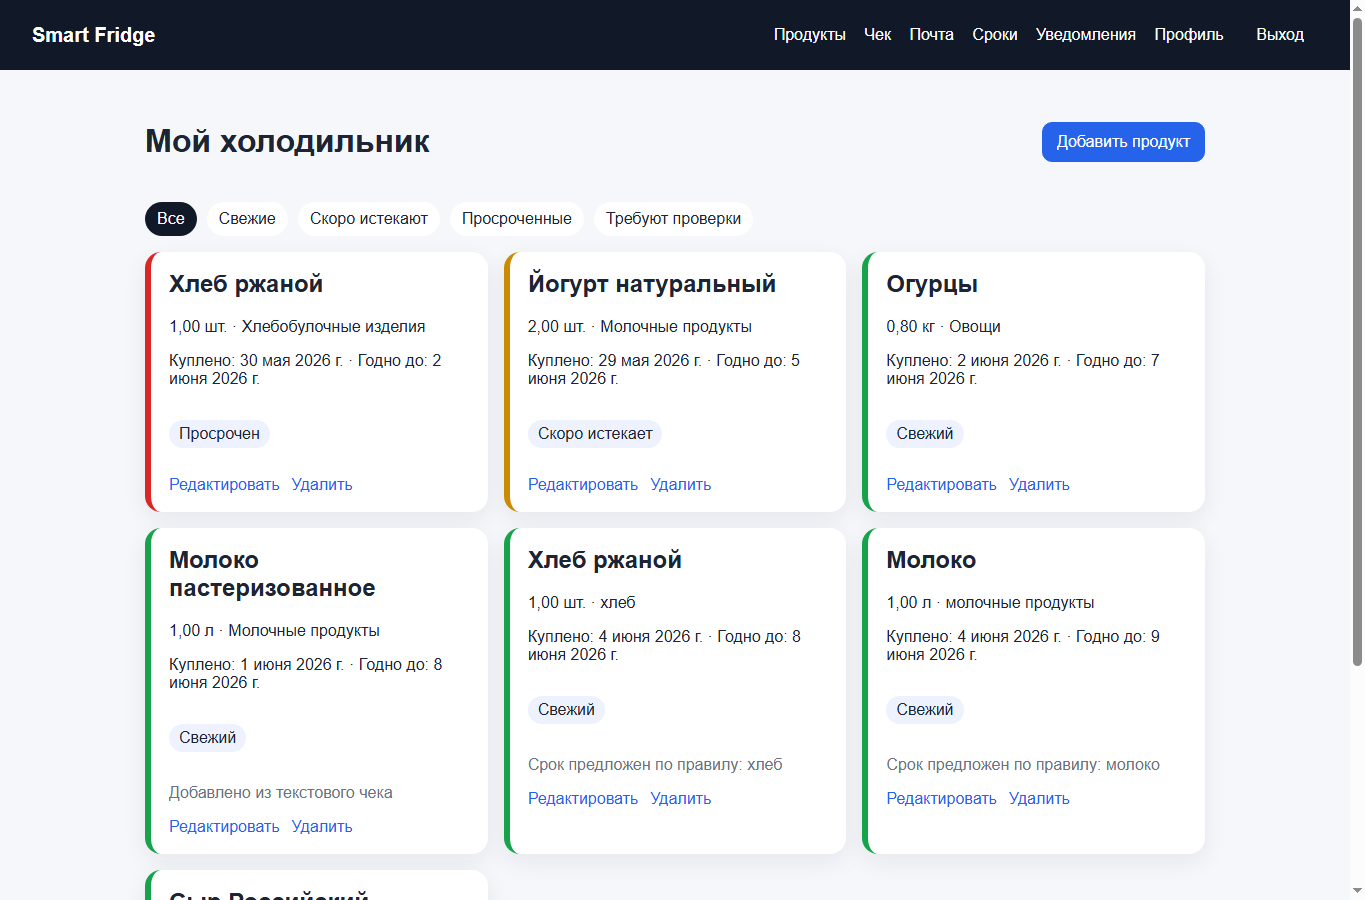
\includegraphics[width=0.95\linewidth]{images/sf_01_products_main.png}
\caption{Главный экран учета продуктов с фильтрацией по состоянию сроков годности}
\label{fig:sf-products-main}
\end{figure}

Главный экран, представленный на рис.~\ref{fig:sf-products-main}, является центральной рабочей областью системы. На нем пользователь видит перечень продуктов, сгруппированный визуально в виде карточек. Каждая карточка содержит название, количество, категорию, дату покупки, дату истечения срока годности и вычисленный статус. Цветовая полоса слева от карточки служит дополнительным индикатором состояния: просроченные позиции выделяются красным, продукты с приближающимся сроком -- предупреждающим цветом, а актуальные продукты -- зеленым.

Над списком расположены фильтры ``Все'', ``Свежие'', ``Скоро истекают'', ``Просроченные'' и ``Требуют проверки''. Эти элементы позволяют быстро перейти от общего перечня к проблемным позициям, требующим внимания пользователя. Кнопка ``Добавить продукт'' переводит к форме ручного ввода, а ссылки ``Редактировать'' и ``Удалить'' на карточках обеспечивают управление отдельными записями без перехода к административной панели Django.

\begin{figure}[H]
\centering
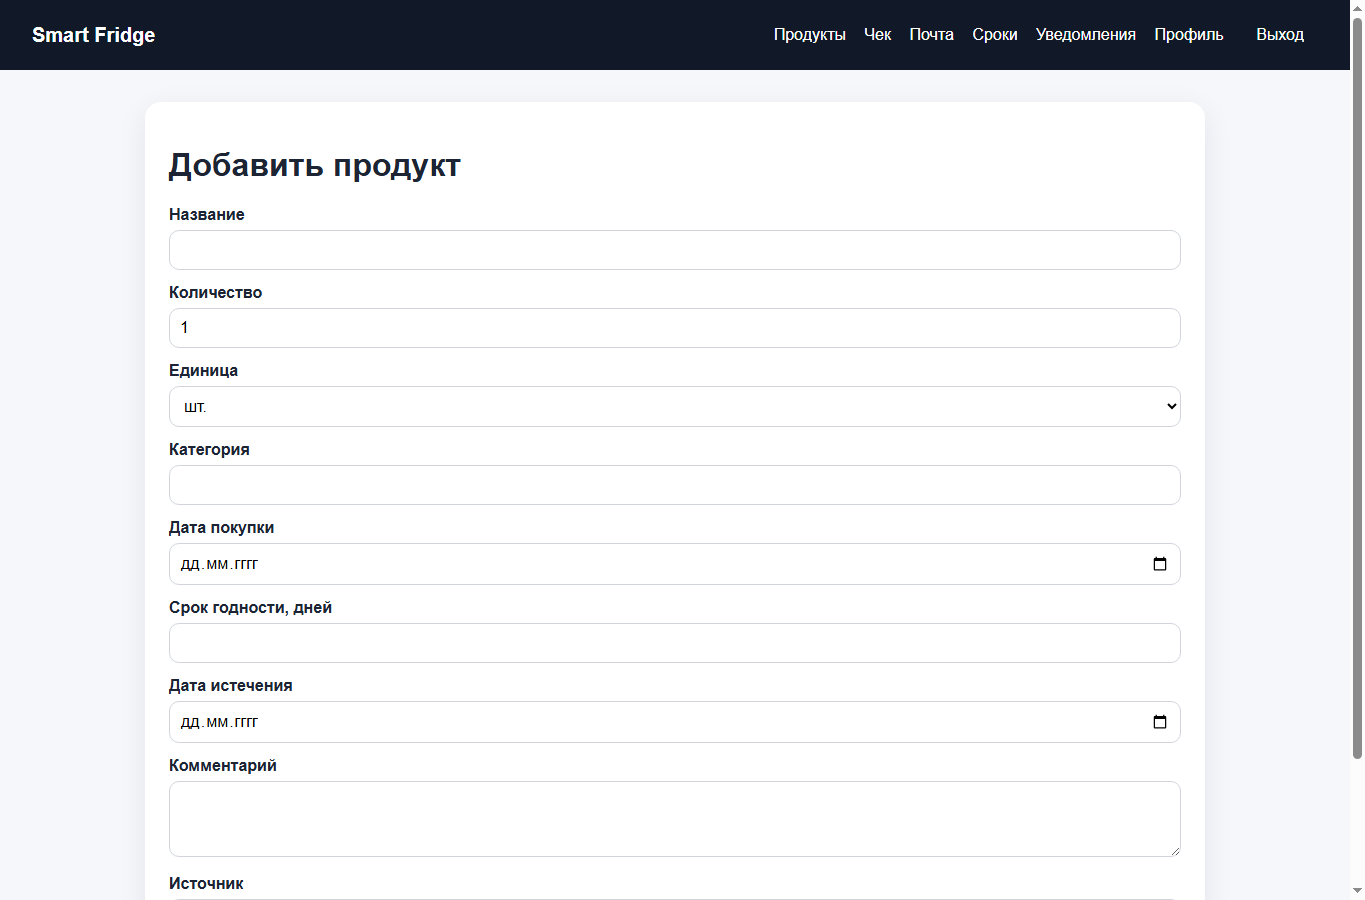
\includegraphics[width=0.95\linewidth]{images/sf_02_product_form.png}
\caption{Форма ручного добавления продукта с параметрами количества, категории и срока хранения}
\label{fig:sf-product-form}
\end{figure}

Форма добавления продукта на рис.~\ref{fig:sf-product-form} используется в сценариях, когда продукт требуется внести без чека или после ручной проверки распознанных данных. Пользователь указывает наименование, количество, единицу измерения, категорию, дату покупки, срок хранения в днях и при необходимости комментарий. Наличие поля источника позволяет системе различать продукты, добавленные вручную, импортированные из чека или полученные из электронной почты.

Если срок хранения не задан пользователем явно, приложение обращается к базе знаний и пытается подобрать подходящее правило по названию продукта. В результате ручной ввод остается достаточно гибким: пользователь может как полностью контролировать параметры записи, так и использовать автоматическую подсказку срока годности на основе уже накопленных правил.

\begin{lstlisting}[style=pythoncode,caption={Фрагмент логики пересчета срока годности}]
def recalculate_expiration(self):
    if self.shelf_life_days is not None:
        self.expiration_date = self.purchase_date + timedelta(days=self.shelf_life_days)

def refresh_status(self):
    if not self.expiration_date or self.shelf_life_days is None:
        self.status = self.STATUS_NEEDS_REVIEW
        return
    today = timezone.localdate()
    if self.expiration_date < today:
        self.status = self.STATUS_EXPIRED
    elif self.expiration_date <= today + timedelta(days=3):
        self.status = self.STATUS_EXPIRING_SOON
    else:
        self.status = self.STATUS_ACTIVE
\end{lstlisting}

\section{Модуль обработки чеков и писем}

Модуль \texttt{receipts} отвечает за получение исходного текста, разбор товарных строк и создание продуктов. В системе предусмотрены три источника: ручной текст, файл чека и электронное письмо. Если внешний OCR-сервис не настроен, файл сохраняется, а пользователь может вручную вставить распознанный текст. Такой fallback повышает надежность учебного проекта.

\begin{figure}[H]
\centering
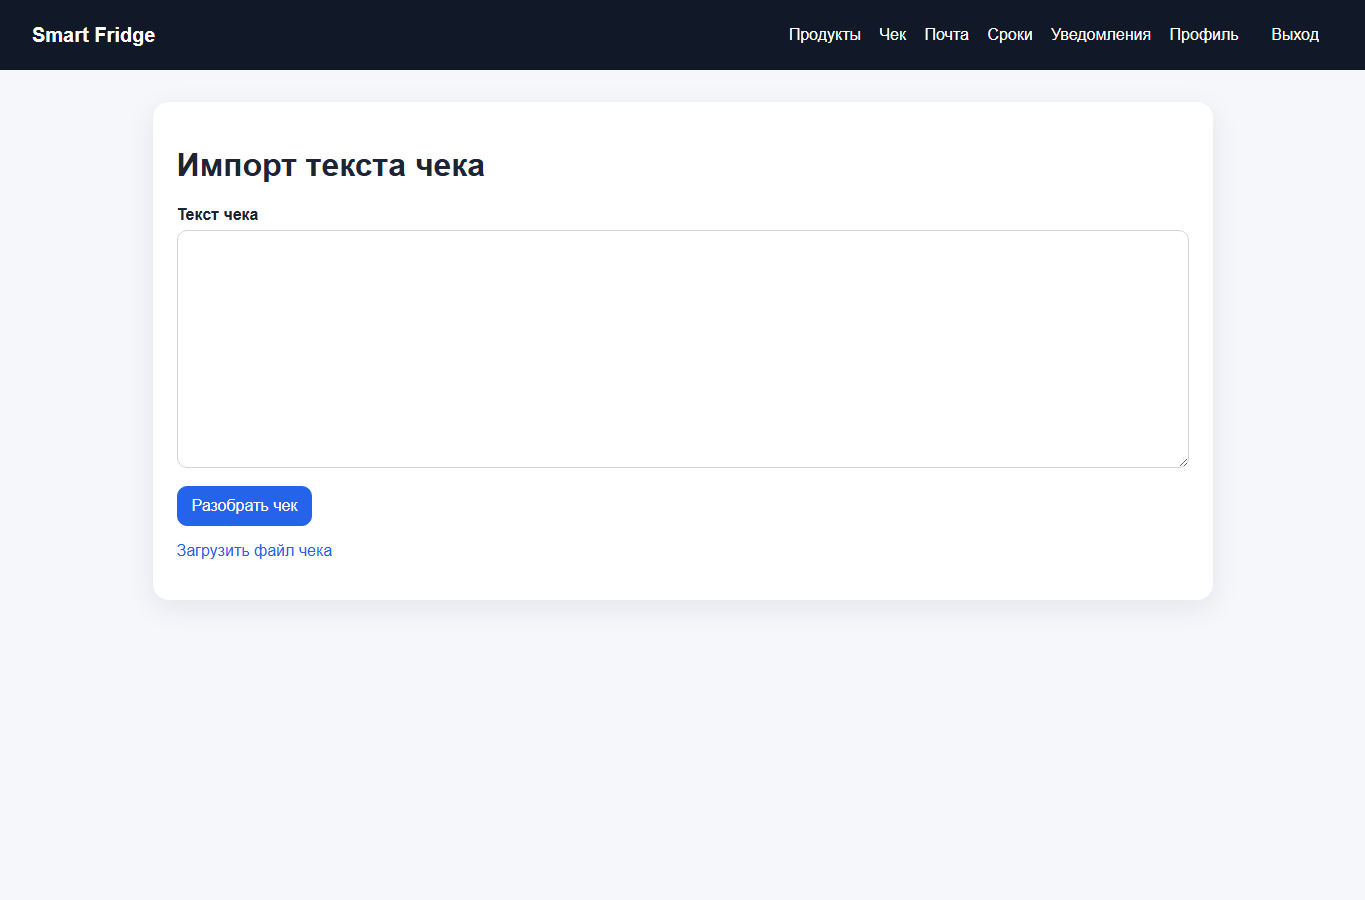
\includegraphics[width=0.95\linewidth]{images/sf_03_receipt_text_form.png}
\caption{Экран ручного импорта текстового представления кассового чека}
\label{fig:sf-receipt-text-form}
\end{figure}

Экран ручного импорта, показанный на рис.~\ref{fig:sf-receipt-text-form}, предназначен для вставки текста чека, полученного из электронного документа, OCR-сервиса или введенного пользователем вручную. Основным элементом страницы является многострочное поле, в котором каждая строка может соответствовать отдельной товарной позиции. После нажатия кнопки ``Импортировать'' данные передаются в сервисный слой, где выполняются очистка текста, извлечение количества и единицы измерения, а также фильтрация непищевых позиций.

Данный сценарий важен для практической эксплуатации, поскольку не зависит от внешних API. Даже при отсутствии подключенного OCR пользователь может внести содержимое чека и получить автоматическое создание продуктовых записей. Это снижает количество ручных действий по сравнению с добавлением каждого продукта через отдельную форму.

\begin{figure}[H]
\centering
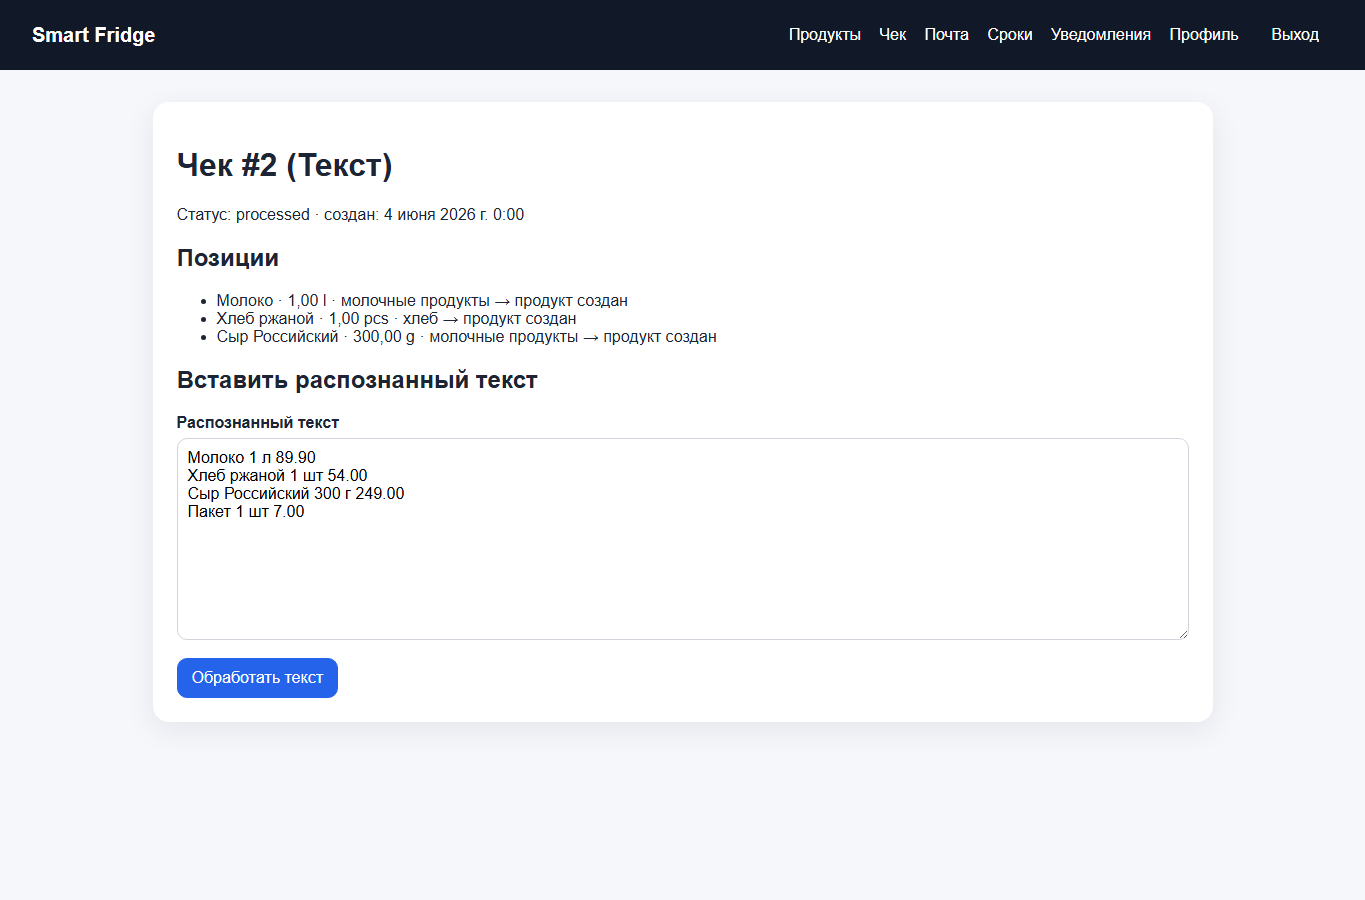
\includegraphics[width=0.95\linewidth]{images/sf_04_receipt_result.png}
\caption{Результат обработки чека с созданными продуктовыми позициями}
\label{fig:sf-receipt-result}
\end{figure}

После обработки чека приложение открывает страницу результата, представленную на рис.~\ref{fig:sf-receipt-result}. На ней фиксируется номер чека, источник данных, статус обработки и дата создания. Ниже отображается перечень распознанных позиций: для каждой строки показаны исходное название, количество, категория и результат создания связанного продукта.

В демонстрационном сценарии система распознала молоко, хлеб и сыр как пищевые товары и создала для них записи в холодильнике. Строка с пакетом используется как пример непищевой позиции, которая не должна превращаться в продуктовый запас. Таким образом, экран результата выполняет контрольную функцию: пользователь может проверить, какие товары были импортированы, и при необходимости повторно обработать распознанный текст.

Почтовый импорт реализован через IMAP. Пользователь задает имя источника, хост IMAP-сервера, порт, логин, пароль приложения, режим SSL и фильтр отправителя или текста. Система проходит по доступным папкам почтового ящика, извлекает текстовые части писем, применяет фильтр и проверяет журнал обработки, чтобы одно письмо не импортировалось повторно.

При обработке письма выполняется очистка текста от недопустимых для PostgreSQL символов, например NUL-байтов. Также система не пытается интерпретировать произвольные бинарные вложения как текст.

\begin{figure}[H]
\centering
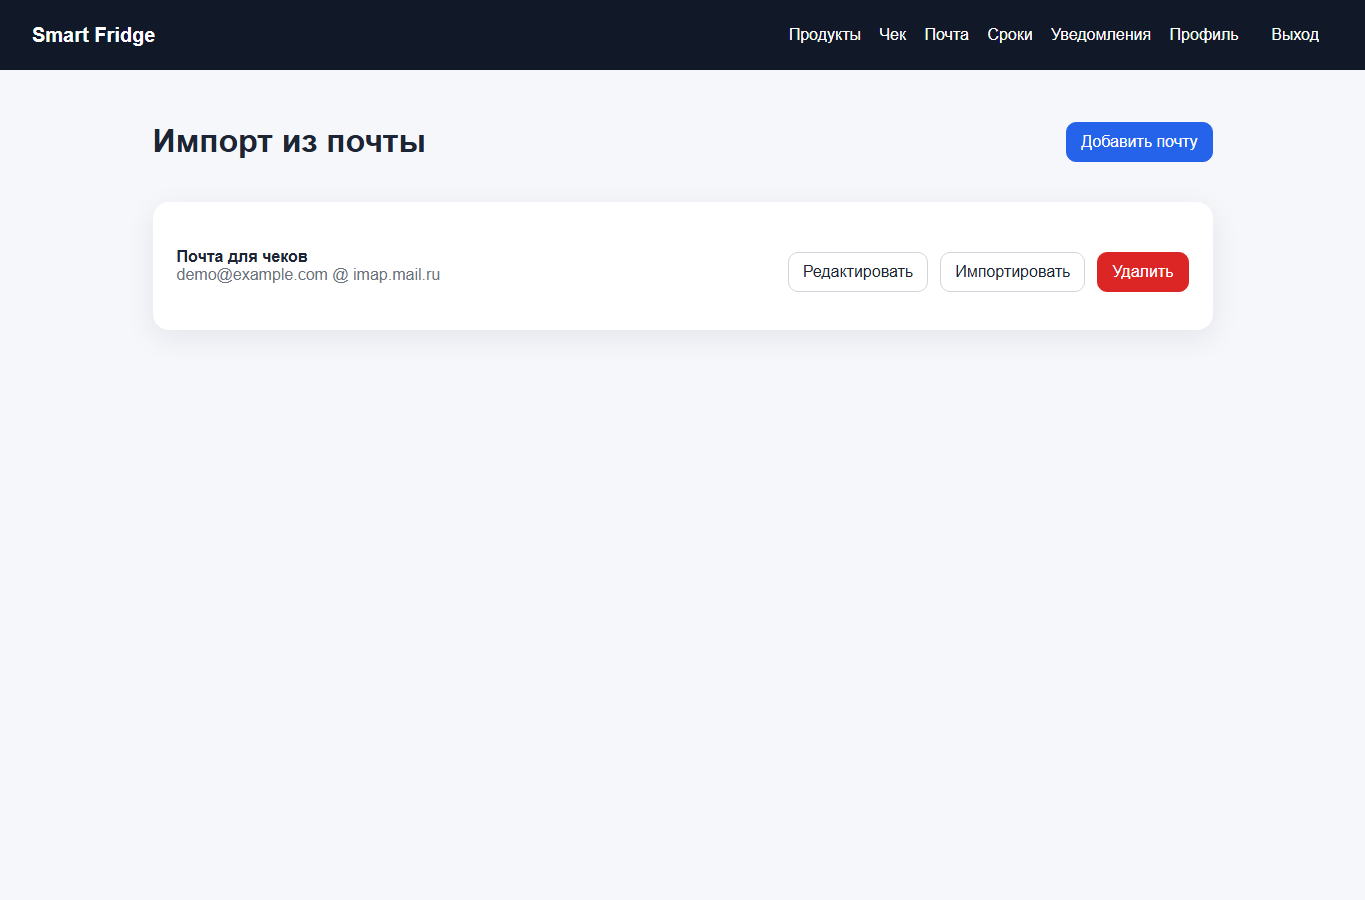
\includegraphics[width=0.95\linewidth]{images/sf_05_email_sources.png}
\caption{Список IMAP-источников для автоматического импорта чеков из электронной почты}
\label{fig:sf-email-sources}
\end{figure}

Раздел почтовых источников на рис.~\ref{fig:sf-email-sources} показывает настроенные подключения к почтовым ящикам. Для каждого источника отображается пользовательское имя, адрес сервера, логин и фильтр, по которому приложение отбирает письма с чеками. Наличие кнопки запуска импорта рядом с источником делает сценарий управляемым: пользователь может инициировать обработку в нужный момент, не обращаясь к командной строке.

На этом же экране доступны операции редактирования и удаления источника. Такая организация интерфейса важна для безопасности и сопровождаемости: пароль приложения и параметры IMAP можно изменить при смене почтового сервиса, а неактуальные источники удалить, чтобы они не участвовали в последующих попытках импорта.

\begin{figure}[H]
\centering
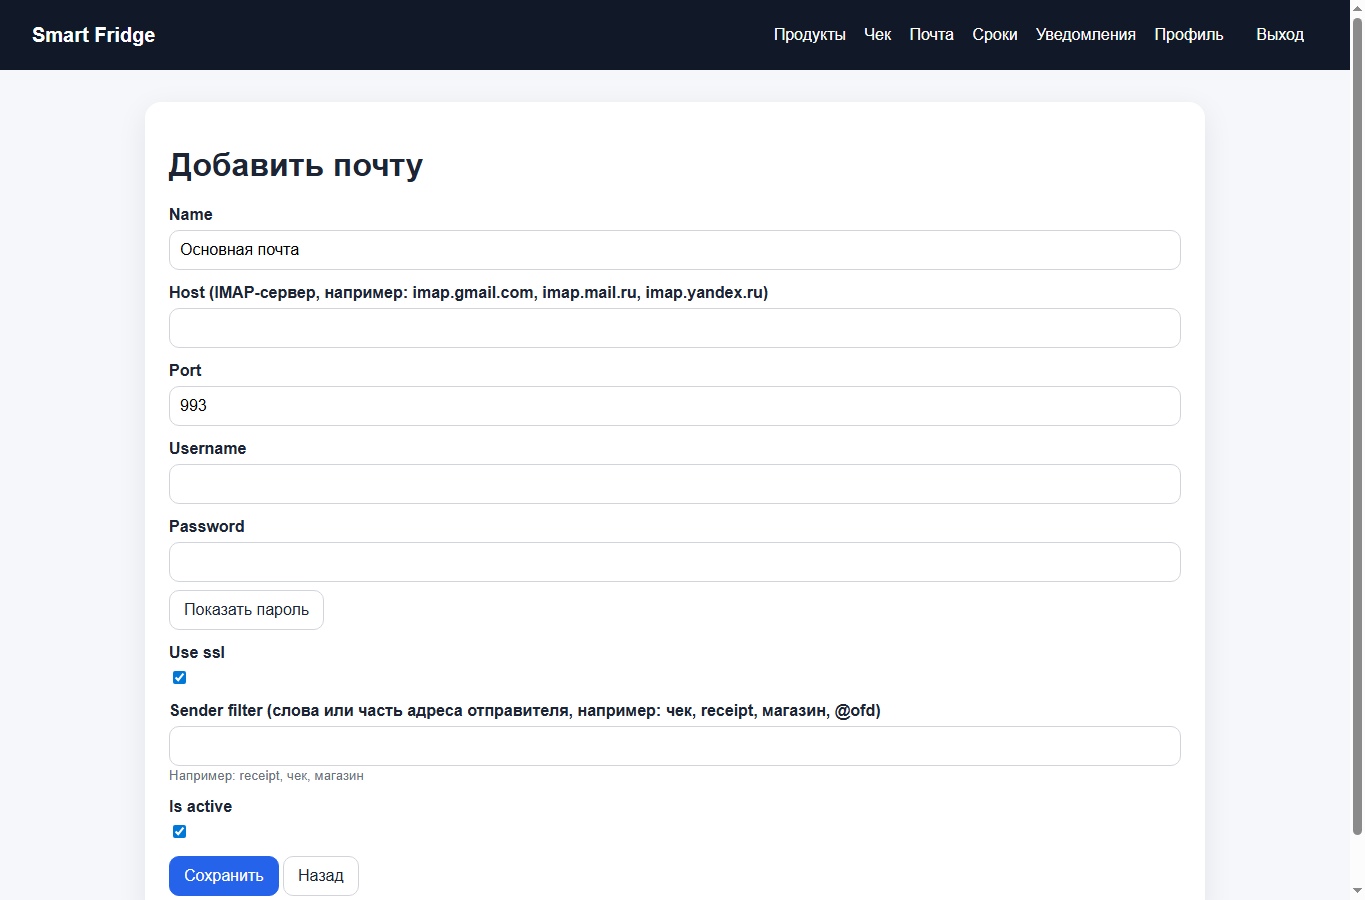
\includegraphics[width=0.95\linewidth]{images/sf_06_email_source_form.png}
\caption{Форма настройки IMAP-подключения и фильтрации писем с кассовыми чеками}
\label{fig:sf-email-source-form}
\end{figure}

Форма добавления почтового источника, показанная на рис.~\ref{fig:sf-email-source-form}, содержит параметры, необходимые для подключения к IMAP-серверу: название источника, хост, порт, учетную запись, пароль приложения, признак использования SSL, фильтр отправителя и признак активности. Поле фильтра позволяет ограничить обработку письмами от магазинов, операторов фискальных данных или сервисов электронных чеков.

Практическая ценность этой формы заключается в том, что пользователь может настроить автоматизированный канал пополнения холодильника без изменения программного кода. В учебном проекте импорт запускается синхронно, однако выбранная структура данных допускает дальнейшее развитие сценария, например перенос запуска в планировщик задач или фоновую очередь.

\section{Модуль базы знаний}

Модуль \texttt{knowledge} хранит правила сроков хранения. Каждое правило содержит название продукта, описание, срок хранения в днях, условия хранения, категорию, теги и признак активности. Правило может быть общим или пользовательским. Пользовательское правило имеет приоритет над общим, что позволяет адаптировать систему под индивидуальные привычки хранения.

Сервис \texttt{ShelfLifeService} сначала ищет точное совпадение названия продукта, затем применяет оценку похожести на основе \texttt{SequenceMatcher} и пересечения токенов. При наличии настроенного внешнего LLM-сервиса возможно уточнение срока хранения на основе найденных кандидатов, однако система остается работоспособной без внешнего API.

\begin{figure}[H]
\centering
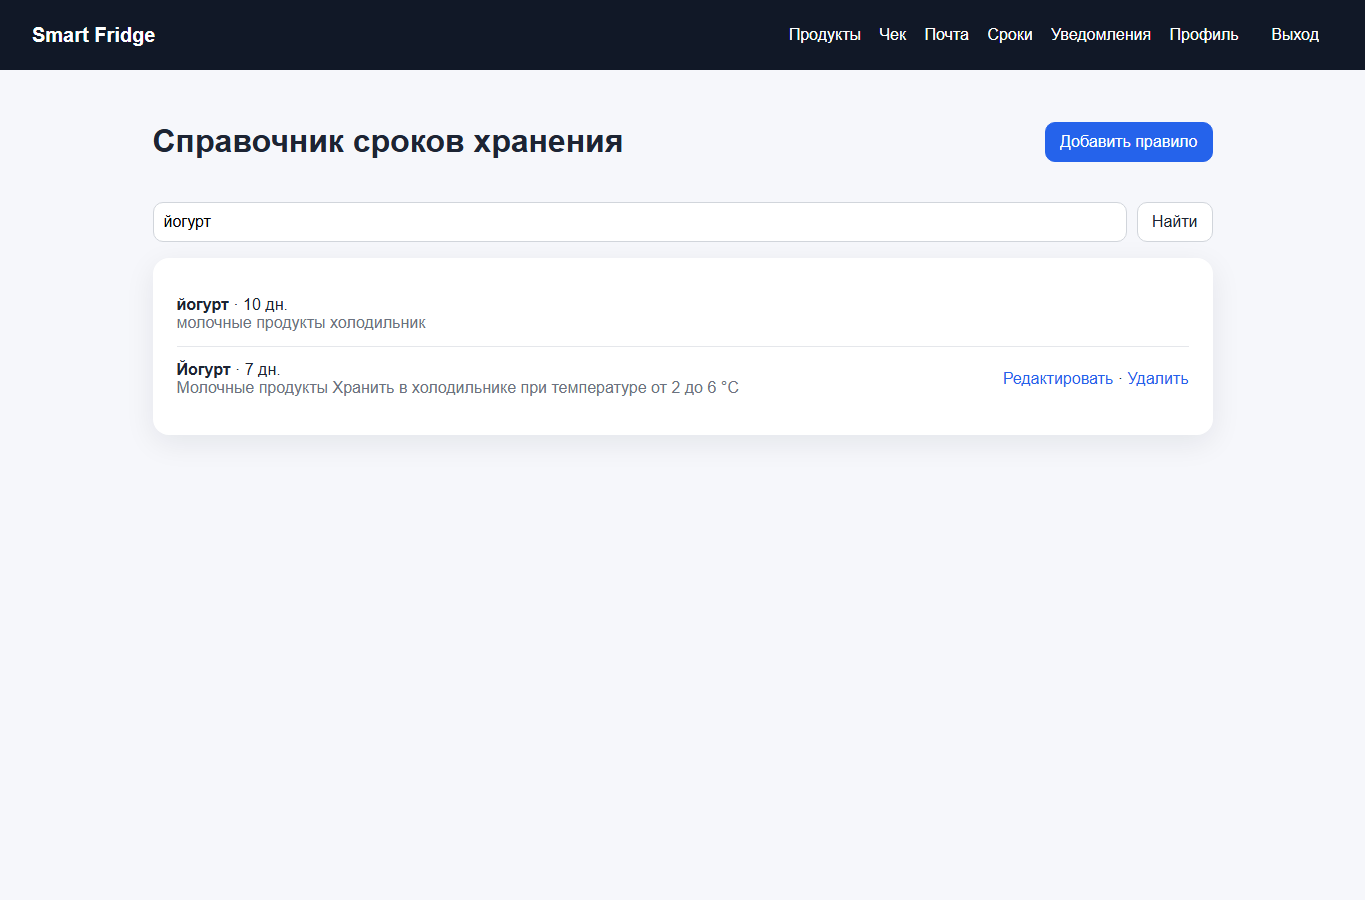
\includegraphics[width=0.95\linewidth]{images/sf_07_knowledge_rules.png}
\caption{Справочник сроков хранения с поиском правил по названию продукта}
\label{fig:sf-knowledge-rules}
\end{figure}

Справочник сроков хранения на рис.~\ref{fig:sf-knowledge-rules} используется для просмотра и поиска правил, по которым приложение предлагает срок годности. В верхней части находится строка поиска по названию продукта или тегам. В демонстрационном примере выполнена фильтрация по слову ``йогурт'', поэтому пользователь видит как общее правило, так и пользовательское правило с индивидуальными условиями хранения.

Наличие нескольких правил по близкому названию показывает механизм приоритета и уточнения. Пользовательская запись может переопределять общий справочник, если в конкретной семье или организации продукт хранится иначе. Это делает систему не только статическим каталогом, но и адаптируемым инструментом поддержки решений.

\begin{figure}[H]
\centering
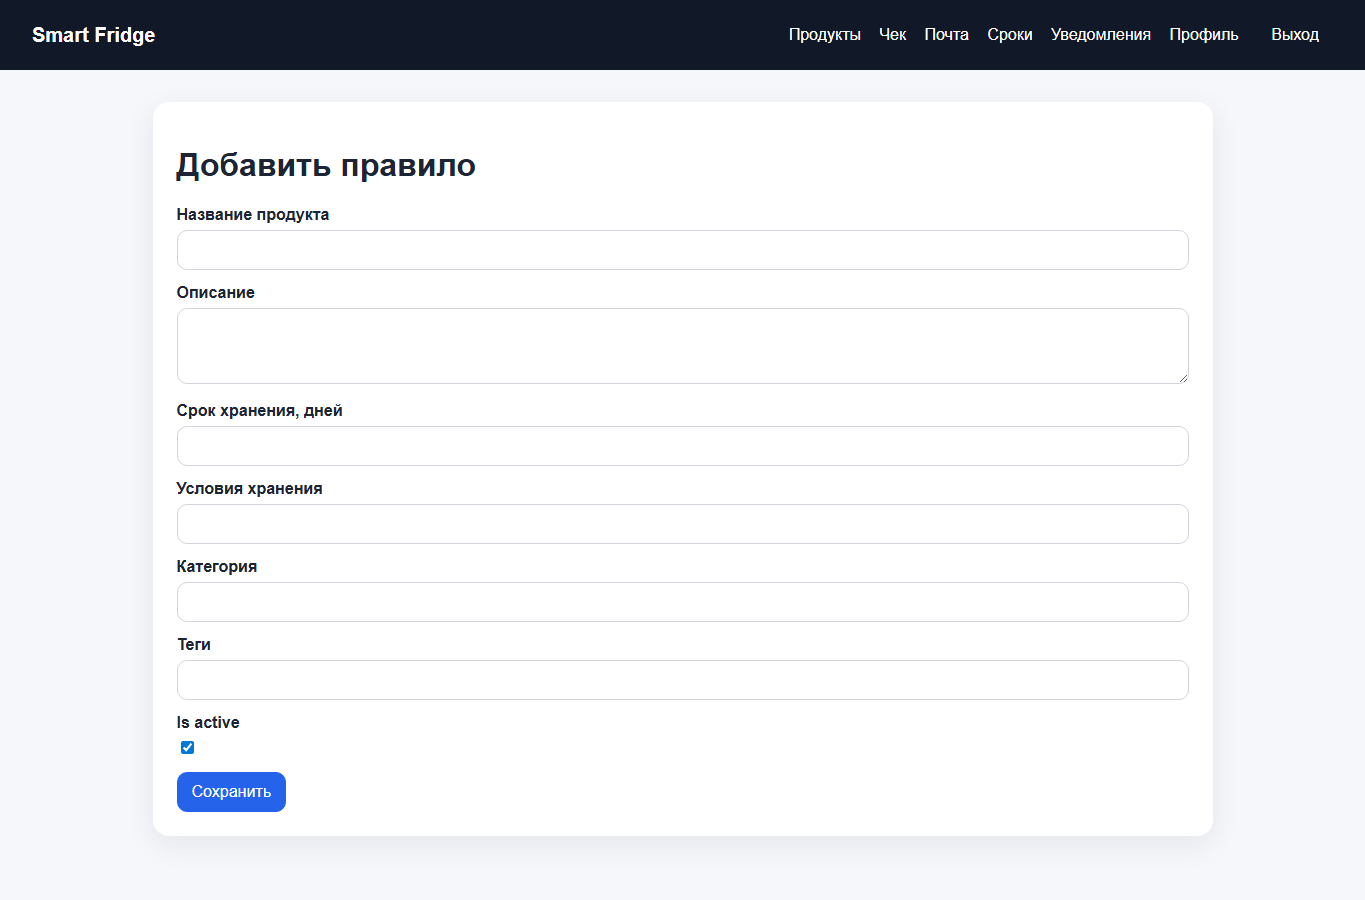
\includegraphics[width=0.95\linewidth]{images/sf_08_knowledge_form.png}
\caption{Форма создания пользовательского правила срока хранения продукта}
\label{fig:sf-knowledge-form}
\end{figure}

Форма создания правила, представленная на рис.~\ref{fig:sf-knowledge-form}, позволяет расширять базу знаний без вмешательства разработчика. Пользователь задает название продукта, описание, срок хранения в днях, условия хранения, категорию, теги и активность правила. Эти поля соответствуют данным, которые затем используются сервисом подбора срока годности при добавлении продуктов.

Особое значение имеют теги и условия хранения. Теги повышают качество поиска и сопоставления похожих названий, а условия хранения объясняют, почему выбран именно такой срок. Благодаря этому приложение не просто автоматически подставляет число дней, а сохраняет контекст принятого решения.

\section{Модуль уведомлений}

Модуль \texttt{notifications} формирует уведомления о сроках годности. Сервис проверяет продукты с известной датой истечения и создает уведомления за 3 дня, за 1 день и после наступления просрочки. Если у пользователя включены email-уведомления и указан адрес, сообщение отправляется через стандартный Django email backend.

Формирование уведомлений вынесено в management command \texttt{generate\_notifications}. Команду можно запускать вручную или по расписанию средствами операционной системы, например через Планировщик задач Windows или cron.

\begin{figure}[H]
\centering
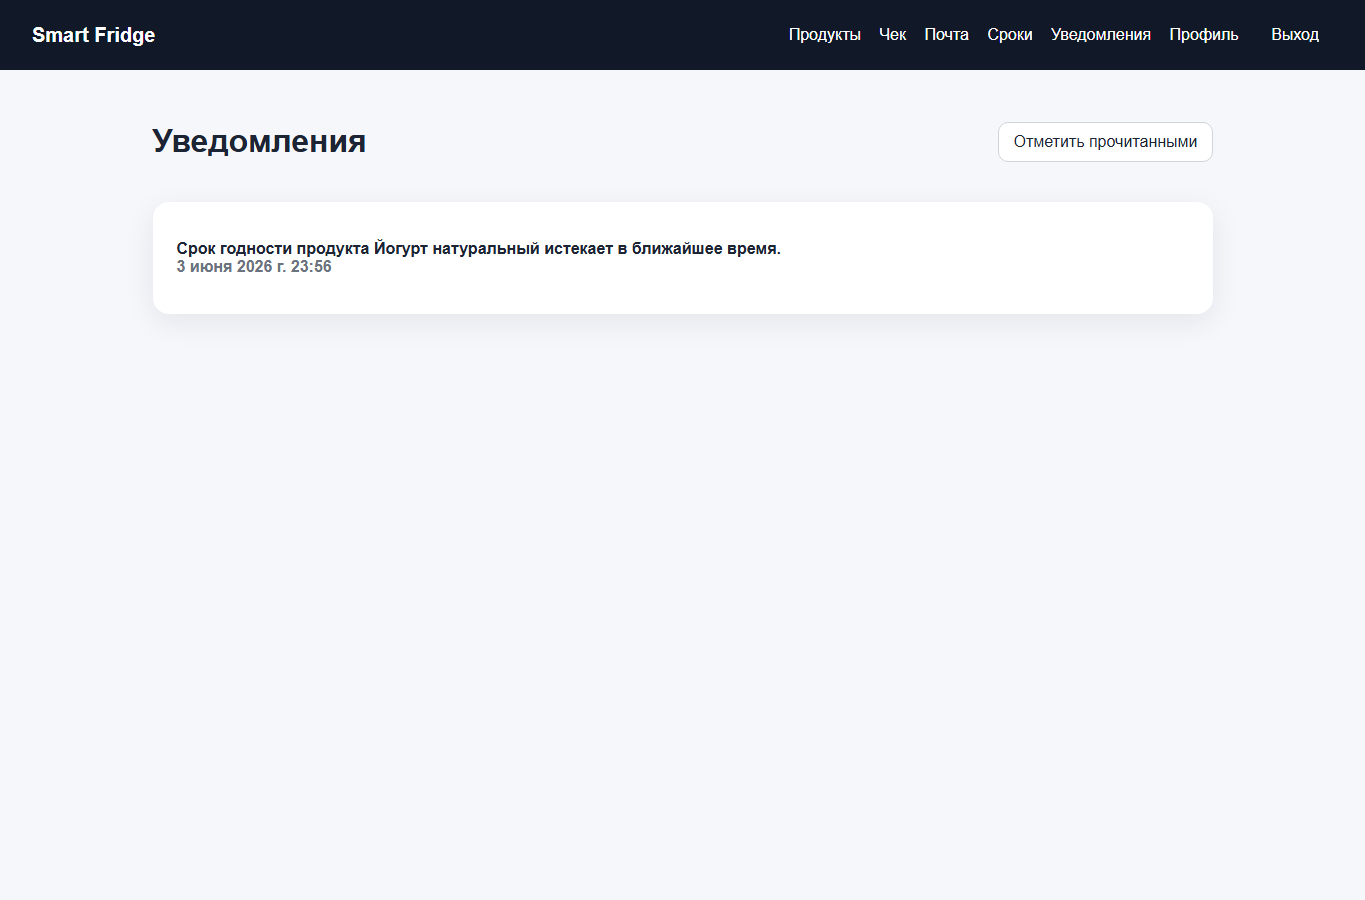
\includegraphics[width=0.95\linewidth]{images/sf_09_notifications.png}
\caption{Раздел уведомлений о приближении или наступлении срока годности продуктов}
\label{fig:sf-notifications}
\end{figure}

Раздел уведомлений на рис.~\ref{fig:sf-notifications} предназначен для концентрации событий, требующих реакции пользователя. В нем отображается текст сообщения, связанный продукт, тип уведомления и признак прочтения. Такой экран дополняет цветовую индикацию на главной странице: даже если пользователь не просматривает весь список продуктов, он может увидеть наиболее важные предупреждения в отдельном разделе.

Кнопка ``Отметить все прочитанными'' переводит уведомления в обработанное состояние. Это удобно при регулярной работе с системой, поскольку пользователь отделяет новые события от уже просмотренных и тем самым снижает риск пропустить продукт с истекающим сроком годности.

\begin{figure}[H]
\centering
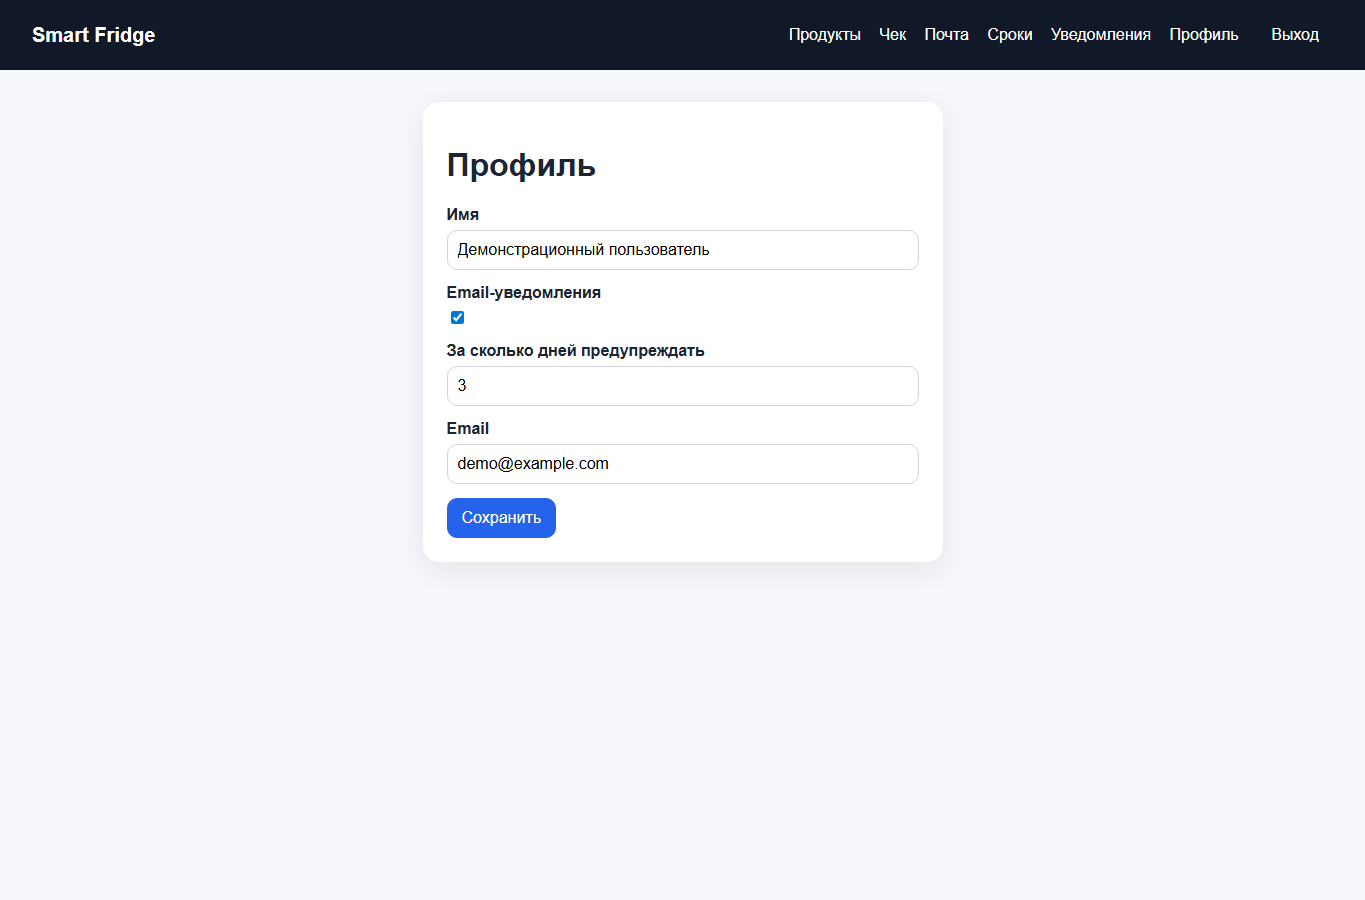
\includegraphics[width=0.95\linewidth]{images/sf_10_profile.png}
\caption{Профиль пользователя с настройками email-уведомлений и горизонта предупреждения}
\label{fig:sf-profile}
\end{figure}

Профиль пользователя, показанный на рис.~\ref{fig:sf-profile}, связывает учетную запись с персональными настройками уведомлений. В форме указываются имя, адрес электронной почты, признак включения email-уведомлений и количество дней до истечения срока, за которое пользователь хочет получать предупреждение. Эти параметры позволяют адаптировать поведение системы под разные бытовые сценарии.

Если email-уведомления отключены, приложение сохраняет предупреждения только во внутреннем разделе. Если они включены и почтовый backend настроен, система может отправлять сообщения на указанный адрес. Таким образом, профиль выступает связующим элементом между учетной записью, системой уведомлений и выбранным пользователем способом получения информации.

\begin{figure}[H]
\centering
\begin{tikzpicture}[
  node distance=1.2cm and 1.2cm,
  screen/.style={rectangle, draw, rounded corners, align=center, minimum width=3.1cm, minimum height=1.0cm},
  arrow/.style={-{Stealth[length=3mm]}, thick}
]
\node[screen] (login) {Вход\\и регистрация};
\node[screen, right=of login] (products) {Список\\продуктов};
\node[screen, right=of products] (product) {Карточка\\продукта};
\node[screen, below=of products] (receipt) {Импорт\\чека};
\node[screen, left=of receipt] (email) {Импорт\\из почты};
\node[screen, right=of receipt] (notify) {Уведомления};
\draw[arrow] (login) -- (products);
\draw[arrow] (products) -- (product);
\draw[arrow] (products) -- (receipt);
\draw[arrow] (email) -- (receipt);
\draw[arrow] (receipt) -- (products);
\draw[arrow] (products) -- (notify);
\end{tikzpicture}
\caption{Основные пользовательские экраны системы}
\label{fig:sf-user-screens}
\end{figure}

Схема на рис.~\ref{fig:sf-user-screens} обобщает рассмотренные пользовательские маршруты. После входа пользователь попадает к списку продуктов, откуда может перейти к карточкам, импорту чеков, настройке почтового источника, базе знаний и уведомлениям. Такая структура соответствует модульной организации Django-приложения и одновременно сохраняет для пользователя единый навигационный контур.

\newpage
\chapter[Глава \thechapter Описание алгоритмов]{Описание алгоритмов}

\section{Алгоритм импорта текста чека}

Алгоритм импорта текста чека состоит из следующих этапов:
\begin{enumerate}
  \item получение исходного текста из формы, файла или письма;
  \item удаление недопустимых символов и нормализация строк;
  \item разбиение текста на отдельные строки;
  \item исключение пустых строк и служебных строк, содержащих слова ``итого'', ``кассир'', ``ИНН'', ``оплата'', ``карта'';
  \item применение регулярного выражения для выделения названия, количества и единицы измерения;
  \item классификация позиции как пищевой или непищевой;
  \item создание записи \texttt{ReceiptItem};
  \item создание записи \texttt{Product} для пищевых позиций.
\end{enumerate}

Регулярное выражение допускает русские и латинские символы, числа, проценты, пробелы и типовые единицы измерения. Это позволяет обрабатывать простые строки чеков вида:
\begin{center}
\texttt{Молоко 1 л 99.00}
\end{center}

\section{Алгоритм классификации продуктовых позиций}

Классификация основана на словарях ключевых слов. Сначала проверяются непищевые признаки: пакет, салфетки, шампунь, мыло, гель, зубная паста, порошок, батарейка, лампа. Если такие слова найдены, позиция исключается. Далее проверяются пищевые признаки: молоко, кефир, сыр, хлеб, курица, рыба, яйцо, яблоко, картофель, рис, макароны, масло, сок и другие.

Такой алгоритм является простым и интерпретируемым. Его преимущество состоит в прозрачности: пользователь и разработчик могут понять, почему строка была добавлена или отклонена. Ограничение подхода состоит в зависимости от полноты словаря, поэтому система может быть расширена за счет пользовательских правил или более сложной модели классификации.

\section{Алгоритм подбора срока хранения}

Подбор срока хранения выполняется в несколько этапов. Сначала сервис ищет активное пользовательское правило с точным совпадением названия продукта. Если пользовательского правила нет, выполняется поиск общего правила. Если точного совпадения нет, из базы выбираются кандидаты и вычисляется оценка похожести:
\[
  S = \max(S_{seq}, S_{tokens}),
\]
где \(S_{seq}\) -- похожесть строк по алгоритму \texttt{SequenceMatcher}, а \(S_{tokens}\) -- доля пересекающихся токенов между названием продукта и текстовыми полями правила.

Кандидаты с оценкой ниже порога отбрасываются. Если внешний LLM-сервис не настроен, выбирается кандидат с наибольшей оценкой. Если подходящего кандидата нет, продукт получает статус, требующий подтверждения.

\section{Алгоритм IMAP-импорта писем}

Алгоритм почтового импорта включает подключение к IMAP-серверу, просмотр папок, получение последних писем, фильтрацию и обработку текста. Для каждого письма формируется внешний идентификатор, состоящий из имени папки и UID письма. Этот идентификатор записывается в \texttt{ProcessingLog}, что предотвращает повторную обработку одного и того же письма.

\begin{lstlisting}[style=pythoncode,caption={Упрощенная схема обработки письма}]
for mailbox in mailboxes:
    connection.select(mailbox, readonly=True)
    ids = connection.search(None, "ALL")
    for uid in ids:
        if already_processed(mailbox, uid):
            continue
        message = fetch_message(uid)
        text = extract_text(message)
        if matches_filter(message, text):
            import_text(text, source="email")
            log_success(mailbox, uid)
\end{lstlisting}

\section{Алгоритм формирования уведомлений}

Для каждого продукта с известной датой истечения вычисляется разница между датой истечения и текущей датой. Если осталось 3 дня или 1 день, создается соответствующее предупреждение. Если дата истечения уже прошла, создается уведомление о просрочке. Уникальное ограничение на пару ``продукт -- тип уведомления'' исключает многократное создание одинаковых сообщений.

\newpage
\chapter[Глава \thechapter Тестирование и результаты]{Тестирование и результаты}

\section{Стратегия тестирования}

Тестирование проекта выполняется средствами стандартного тестового фреймворка Django. Тесты размещены в каталоге \texttt{tests} и охватывают ключевые сценарии: регистрацию и вход пользователя, создание продукта, обработку чеков, импорт писем, работу базы знаний и генерацию уведомлений.

Особое внимание уделяется сервисам, так как именно они содержат основную бизнес-логику. Для IMAP-импорта используется мокирование класса \texttt{imaplib.IMAP4\_SSL}, что позволяет проверять поведение без реального подключения к почтовому серверу.

\section{Проверенные сценарии}

\begin{enumerate}
  \item Парсинг текста ``Молоко'', ``Пакет'', ``Хлеб'': продукты питания добавляются, непищевая позиция исключается.
  \item Импорт текста чека вручную: создаются записи продуктов для распознанных пищевых строк.
  \item Очистка текста от NUL-байтов: текст сохраняется в PostgreSQL без ошибки.
  \item Повторный импорт письма с тем же UID: письмо пропускается, дубли не создаются.
  \item Редактирование настроек почты: сохраняются новые host, username и sender filter.
  \item Кириллический фильтр отправителя: фильтр применяется внутри Python без ASCII-ошибок IMAP.
  \item Импорт из пользовательской папки почты: письмо находится не только во входящих, но и в других IMAP-папках.
\end{enumerate}

\section{Результаты практической проверки}

Практическая проверка показала, что приложение выполняет основные функции учета продуктов. Ручной импорт текстового чека создает продукты из строк ``Молоко'', ``Хлеб'', ``Сыр'' и исключает строку ``Пакет''. Почтовый импорт способен подключаться к Mail.ru через IMAP при использовании пароля приложения, обрабатывать письма из папки ``Чеки'' и применять фильтр по отправителю, теме или тексту письма.

В ходе проверки были выявлены и устранены типовые проблемы интеграции: необходимость использования пароля приложения для Mail.ru, различие между адресом почты и IMAP-хостом, обработка кириллических фильтров, чтение писем из пользовательских папок и очистка текста от NUL-символов перед сохранением в PostgreSQL.

\section{Ограничения реализации}

Текущая реализация является учебным прототипом и имеет ряд ограничений. Импорт почты запускается вручную пользователем через кнопку ``Импортировать''. Для автоматического запуска требуется добавить отдельную management command и настроить ее выполнение по расписанию. Классификация продуктов основана на словарях, поэтому неизвестные названия могут не распознаваться. OCR и LLM являются необязательными расширениями и используются только при наличии соответствующих переменных окружения.

Несмотря на ограничения, архитектура проекта допускает развитие: расширение словаря продуктов, добавление новых правил сроков хранения, подключение OCR-сервиса, автоматизация импорта и улучшение пользовательского интерфейса.

\newpage
\conclusion

В ходе выполнения курсового проекта была рассмотрена и описана информационная система Smart Fridge, предназначенная для учета продуктов питания, анализа чеков и контроля сроков годности. В теоретической части изучены особенности предметной области, задачи обработки чеков и подходы к автоматическому определению сроков хранения. В аналитической части сформулированы функциональные и нефункциональные требования, обоснован выбор монолитной архитектуры на Django и описана модель данных.

Практическая часть показала, что проект реализует основные функции: регистрацию пользователей, учет продуктов, импорт чеков из текста, файлов и электронной почты, ведение базы знаний сроков хранения и формирование уведомлений. Сервисный слой отделяет бизнес-логику от представлений Django, что повышает сопровождаемость системы.

В работе описаны ключевые алгоритмы: разбор текста чека регулярными выражениями, словарная классификация пищевых товаров, подбор срока хранения по базе знаний, IMAP-импорт писем и генерация уведомлений. Тестирование подтвердило работоспособность основных сценариев и устойчивость к ряду практических ошибок, возникающих при обработке электронной почты.

Таким образом, цель курсового проекта достигнута: разработана и описана информационная система учета продуктов питания с анализом чеков и контролем сроков годности. Полученный прототип может быть использован как основа для дальнейшего развития, включая автоматический импорт писем по расписанию, расширение базы знаний и применение более точных методов распознавания товарных позиций.

\newpage
\renewcommand\bibname{\centering Библиографический список}
\clearpage
\addcontentsline{toc}{chapter}{Библиографический список}
\begin{thebibliography}{99}
\bibitem{django} Django documentation [Электронный ресурс]. -- Режим доступа: https://docs.djangoproject.com/ -- Заглавие с экрана. -- (Дата обращения: 29.05.2026).
\bibitem{postgresql} PostgreSQL Documentation [Электронный ресурс]. -- Режим доступа: https://www.postgresql.org/docs/ -- Заглавие с экрана. -- (Дата обращения: 29.05.2026).
\bibitem{python} Python 3 Documentation [Электронный ресурс]. -- Режим доступа: https://docs.python.org/3/ -- Заглавие с экрана. -- (Дата обращения: 29.05.2026).
\bibitem{imap} Crispin, M. Internet Message Access Protocol -- Version 4rev1 [Электронный ресурс]. -- Режим доступа: https://www.rfc-editor.org/rfc/rfc3501 -- Заглавие с экрана. -- (Дата обращения: 29.05.2026).
\bibitem{gost} ГОСТ Р 7.0.100--2018. Библиографическая запись. Библиографическое описание. Общие требования и правила составления. -- Москва: Стандартинформ, 2018. -- 124 с. -- Текст: непосредственный.
\bibitem{sommerville} Соммервилл, И. Инженерия программного обеспечения / И. Соммервилл. -- 10-е изд. -- Москва: Вильямс, 2016. -- 928 с. -- Текст: непосредственный.
\bibitem{db} Коннолли, Т. Базы данных. Проектирование, реализация и сопровождение. Теория и практика / Т. Коннолли, К. Бегг. -- 3-е изд. -- Москва: Вильямс, 2003. -- 1440 с. -- Текст: непосредственный.
\bibitem{testing} Майерс, Г. Искусство тестирования программ / Г. Майерс, Т. Баджетт, К. Сандлер. -- 3-е изд. -- Москва: Диалектика, 2012. -- 272 с. -- Текст: непосредственный.
\bibitem{ocrbook} Гонсалес, Р. Цифровая обработка изображений / Р. Гонсалес, Р. Вудс. -- 3-е изд. -- Москва: Техносфера, 2012. -- 1104 с. -- Текст: непосредственный.
\end{thebibliography}

\newpage
\applications

\section*{Приложение А. Фрагмент структуры проекта}
\addcontentsline{toc}{section}{Приложение А. Фрагмент структуры проекта}

\begin{lstlisting}[basicstyle=\small\ttfamily,frame=single,breaklines=true]
smart_fridge/
  accounts/       registration and profile
  pantry/         products and categories
  receipts/       receipt parsing and email import
  knowledge/      shelf-life rules
  notifications/  expiration notifications
  templates/      Django templates
  tests/          key scenario tests
\end{lstlisting}

\section*{Приложение Б. Пример тестового чека}
\addcontentsline{toc}{section}{Приложение Б. Пример тестового чека}

\begin{quote}
\small\ttfamily
Молоко 1 л 99.00\\
Хлеб 1 шт 55.00\\
Сыр 1 шт 180.00\\
Пакет 1 шт 7.00
\end{quote}

\end{document}
